\documentclass{sig-alternate}%[conference][letterpaper]
\usepackage{times,amsmath}
\usepackage{epsfig,algorithm,caption,subcaption,multirow}
\usepackage[noend]{algpseudocode}
\usepackage[normalem]{ulem}
\usepackage{color,url}
\usepackage{balance}
\DeclareCaptionType{copyrightbox}

\newcommand{\secref}[1]{Section \ref{#1}}
\newcommand{\figref}[1]{Figure \ref{#1}}
\newcommand{\equref}[1]{Equation (\ref{#1})}
\newcommand{\exref}[1]{Example \ref{#1}}

\newcommand{\KZ}[1]{\textcolor{green}{[KZ: #1]}}
\newcommand{\HAIXUN}[1]{\textcolor{red}{[HAIXUN: #1]}}
\newcommand{\myurl}[1]{\textsf{{\uline{#1}}}}

\newcommand{\cut}[1]{}
\newcommand{\myskip}{\vspace*{1ex}}
\newcommand{\shrink}{\vspace*{-1ex}}

%\theoremstyle{definition}
%\newenvironment{example}[1][Ex.]{\begin{trivlist}
%\item[\hskip \labelsep {\bfseries #1}]}{\end{trivlist}}
\newtheorem{example}{Example}

\newcommand{\lbb}{{\color{black} \textbf{[}}}
\newcommand{\rbb}{{\color{black} \textbf{]}}}
%
%
\newfont{\mycrnotice}{ptmr8t at 7pt}
\newfont{\myconfname}{ptmri8t at 7pt}
\let\crnotice\mycrnotice
\let\confname\myconfname
\conferenceinfo{CIKM'13,}{Oct. 27--Nov. 1, 2013, San Francisco, CA, USA.}
\copyrightetc{Copyright 2013 ACM \the\acmcopyr}
\crdata{978-1-4503-2263-8/13/10\ ...\$15.00.\\
http://dx.doi.org/10.1145/2505515.2505521}
\clubpenalty=10000
\widowpenalty = 10000

\begin{document}
%\conferenceinfo{EDBT'13,} {Mar 18-22, 2013, Genoa, Italy.}
%\CopyrightYear{2013}
%\crdata{978-1-4503-1462-6 /12/08}
%\clubpenalty=10000
%\widowpenalty = 10000
\title{Wikification via Link Co-occurrence}

\numberofauthors{3}
\author{%
\alignauthor
Zhiyuan Cai \hspace*{3mm} Kaiqi Zhao\\
	\affaddr{Shanghai Jiao Tong University}\\
	\affaddr{Shanghai, China}\\
    \affaddr{\{luckyvega,kaiqi\_zhao\}@sjtu.edu.cn}
    %\email{\small \{luckyvega,kaiqi\_zhao\}@sjtu.edu.cn}
	%\email{luckyvega,kaiqi\_zhao@sjtu.edu.cn}
    %\affaddr{\small \{luckyvega,kaiqi\_zhao\}@sjtu.edu.cn}
    %\affaddr{\{luckyvega,kaiqi\_zhao\}@sjtu.edu.cn}
\alignauthor
Kenny Q. Zhu\\
	\affaddr{Shanghai Jiao Tong University}\\
	\affaddr{Shanghai, China}\\
    \affaddr{kzhu@cs.sjtu.edu.cn}
	%\affaddr{\small kzhu@cs.sjtu.edu.cn}
\alignauthor
Haixun Wang\\
	\affaddr{Google Research}\\
	\affaddr{Mountainview, CA, USA}\\
    \affaddr{haixun@google.com}
	%\affaddr{\small haixun@google.com}
}
\maketitle

\begin{abstract}
Wikification, which stands for the process of linking terms in a
plain text document to Wikipedia articles which represent the correct
meanings of the terms, can be thought
of as a generalized Word Sense Disambiguation problem.
It disambiguates multi-word expressions (MWEs) in addition to single words.
Existing Wikification techniques either models the context of a given
term as well as the Wikipedia article as bags of words, or compute
global constraints among Wikipedia concepts by the link graph or
link distributions. The first method doesn't achieve good results
because the MWEs can have very different meanings than its constituent
words which themselves are ambiguous. The second method doesn't produce
high accuracy because the link structure or link distribution is often
biased or incomplete by themselves due to the fact that Wikipedia pages
are often sparsely linked.
In this paper, we present a simple but powerful framework
of sense disambiguation
using co-occurrences of Wikipedia links in the Wikipedia
corpus. We propose an iterative method to enrich the sparsely-linked
articles by adding more links and then use the resulting
link co-occurrence matrix to disambiguate an input document by a sliding
window algorithm.  Our prototype system achieves 89.97\% precision
and 76.43\% recall on average for three benchmark data and
compares favorably against four state-of-the-art wikification techniques.
\footnote{Kenny Q. Zhu (corresponding author) is partially
supported by NSFC grants 61100050 and 61373031.}
\end{abstract}

\category{I.2.7}{ARTIFICIAL INTELLIGENCE}{Natural Language Processing}

% NOTE keywords are not used for conference papers so do not populate them
\begin{keywords}
Wikification; phrase sense disambiguation; link co-occurrence; iterative
algorithm
\end{keywords}
\setlength{\floatsep}{2.2mm plus 1mm minus 1mm}
\setlength{\textfloatsep}{2.2mm plus 1mm minus 1mm}
\setlength{\intextsep}{2.2mm plus 1mm minus 1mm}
\section{Introduction}

Protein$-$protein interactions (PPIs) are of central importance for the majority of biological functions, such as signal transduction, metabolic pathways, molecular dynamics, and protein networks\cite{Hoffmann.Krallinger.ea:2005}, for they serve as the most fundamental building blocks of the entire interacademic systems of any organisms. Collecting data on pairwise interaction relationships is essential for multiple purpose, including identification of modules with certain functionality\cite{Spirin.Mirny.03}, mapping diseases to dominated genes\cite{Ideker.Sharan.08}, and after all, understanding wholistic metabolic/genetic networks from a system biology perspective.

A lot of databases have been built to store protein and genetic interactions from major model organism species and are available in various standardized formats, such as MINT\cite{Zanzoni.Montecchi-Palazzi.ea:2002}, BIND\cite{Bader.ea:2003}, BIOGRID\cite{DBLP:journals/nar/StarkBRBBT06}, etc. Among those mainstream databases, the data largely rely on voluntary reports by scientists or researchers, besides, comprehensive curation efforts become indispensable for the sake of accuracy. However, the amount of biology-related literatures with respect to protein interactions grows explosively and thus make it either impossible or impractical to manually detect PPI information anymore.

Considering huge amount of PPI information with great wealth hidden in published papers, in recent years, numerous mining techniques have been proposed that aim to extract PPI information automatically from free text, especially machine learning, information retrieval, and natural language processing\cite{DBLP:journals/bib/WinnenburgWPDS08}.These approaches can be roughly categorized into three classes: co$-$occurrence, rule$-$based, and machine learning. 

Co$-$occurrence is the approach with most simplicity and naivete. Just as its name implies, this method intends to find out pairs of proteins that co-occur in the same context. The scope of "same context" ranges from phrase, sentence, paragraph to whole abstract, even document. The underlying assumption is that whenever two proteins are mentioned together by authors, chances are high that there is some kind of relationship between them. However, however, in-context closeness even semantic relation does not necessarily represent actual biological interaction. As a consequence, a large fraction of candidate pairs are mismatched inevitably, causing a high recall but low precision.

The second approach is rule-based extraction, in other words, pattern matching. There are many types of rules, most of them concern natural language processing (NLP). One way is to specify hand-crafted regular expressions before hand, which mostly lean on language usage preference. Besides, by using full or partial (shallow) parsing strategies, more information would be acquired, such as part-of-speech taggers, local dependencies between syntactic components, context-free grammar\cite{DBLP:journals/bioinformatics/TemkinG03}, and full sentence structure. Compared to co$-$occurrence, rule-based approach enjoy better precision but much lower recall. In addition, since the rules are usually derived from training data, that is to say, the improper choice of training data would be significantly lethal, therefore quality of extraction is invariably instable and may not applicable to other data.

The third and most commonly used approach use machine learning techniques, in this case, the task to extract protein$-$protein interactions turns out to be a binary classification problem. Each protein pairs are represented along with a set of features, which is associated with their context, then a well$-$defined classifier gives the answer whether the candidate protein pairs is classified to be qualified PPI. (TO BE FURTHER FILLED!!!)

In this paper, we introduce a general bootstrapping framework for Protein$-$protein interaction extraction from natural text.Our method differs from most of the previous works in three aspects:

(1)The extraction process is driven by only tiny fraction of training data, which are regarded as seed data. In each round, it would derive reliable patterns automatically from seed data, then extract more positive PPI pairs consequently, what's more, the seed data would be augmented by the newly extracted results with high confidence.

(2)multiple graph kernel. 

(3)various evaluation.




%\subsection{Model Overview}

In this section, we describe our joint model for cross-lingual table linking.
%\figref{fig:overview} gives a general view of our neural network based joint model.
\figref{fig:overview} gives a general view of the model.
The reason we call it a ``joint model'' is that
the input of neural network is a mention table $X$ containing all the cells to be linked,
together with one candidate entity table $E$,
%All the mentions in the table will be linked simultaneously.
and the output stands for the relevance score $S(X, E)$.
%which indicates the probability of choosing that candidate entity table as final result.

Specifically, we first generate candidate entities of each single mention (\secref{sec:candgen}),
then we learn two different features:
the \textbf{m}ention feature and \textbf{c}ontext feature
derived from the mention-entity embedding pairs of the table (\secref{sec:cell}).
To make different representations from two language spaces compatible,
we utilize a bilingual translation matrix to transform the vector representation
from Chinese to English (\secref{sec:translation}).
Meanwhile, we learn a third feature called \textbf{coh}erence feature
only from the candidate entity table (\secref{sec:coherence}).
%We combine these three features together to calculate the overall relevance score, and finally
Finally, we discuss the prediction and parameter learning step of this task (\secref{sec:strategy}). 

\begin{figure*}
	\centering
	%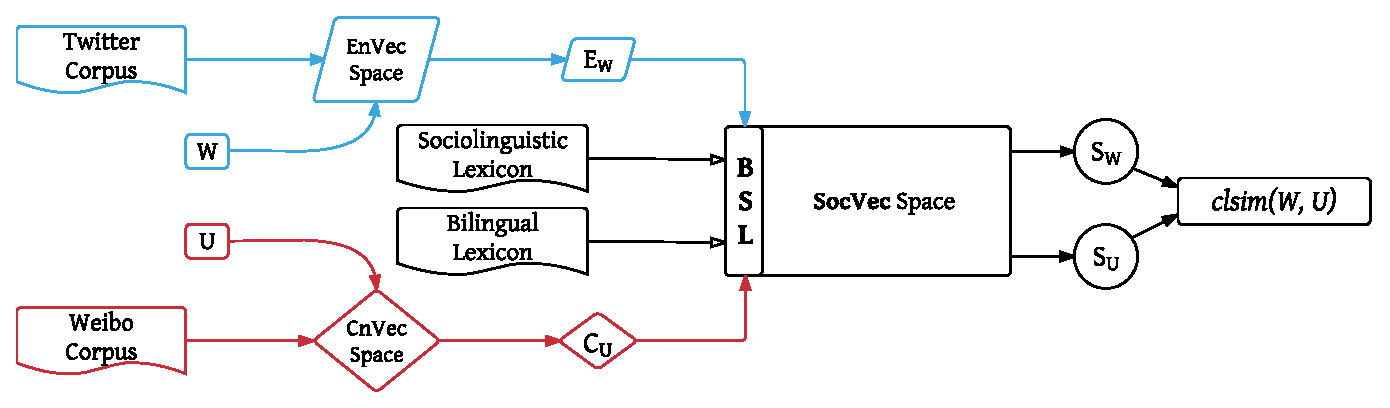
\epsfig{file=figures/overview.eps, angle=0, width=2.0\columnwidth}
	\scalebox{0.28}{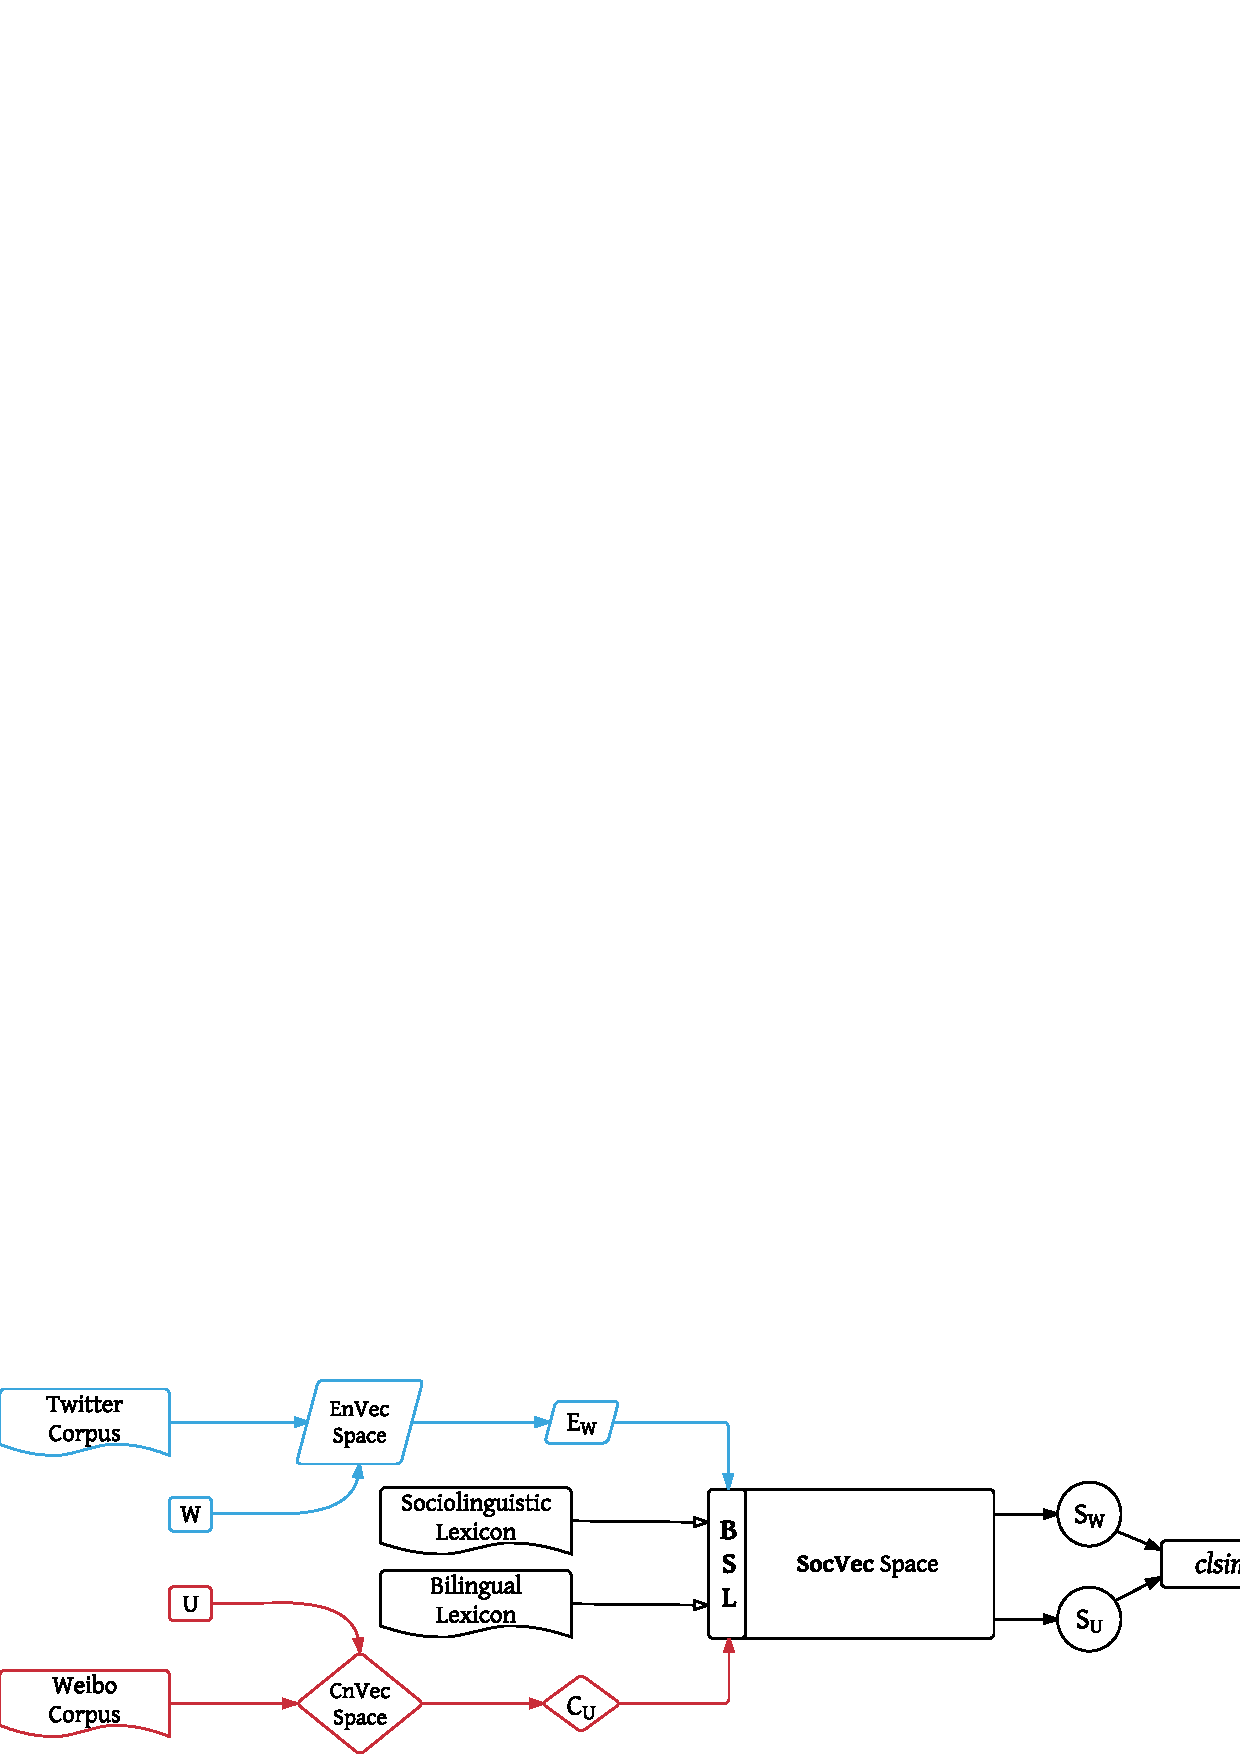
\includegraphics{figures/overview.pdf}}
	\caption{Overview of proposed neural network based joint model.}
	\label{fig:overview}
\end{figure*}

\subsection{Preprocessing}
In this sub-section,we describe the preprocessing step
on Wikipedia corpus.
%\KZ{Why both wiki and plain text, don't we only iterate on wiki docs here?}
We start from the generation
of the term-sense mapping from Wikipedia corpus.
Then we introduce our parsing method on
Wikipedia articles by making use of an NLP chunker.

\subsubsection{Generate Term-Sense Mapping}
%\KZ{Why do we need the candidate sense list?}
To identify the sense of an unlinked term, we need to know the candidate
senses of that term.
Each term may map to more than
one Wikipedia concepts which are the {\em senses}.
%In the following discussion, we will use the term {\em senses}
%and {\em concepts} interchangeably.
The list of all Wikipedia concepts associated with an unlinked term is called
the candidate sense list.
In this paper, we use three sources in Wikipedia to build the
term-sense mapping:
Wikipedia article titles, redirect pages and disambiguation pages.
For each Wikipedia concept (sense), the three kinds of terms that extracted from
%We collect the surface form of a Wikipedia concept/sense from
the title of this concept,
title of redirect pages linked to this concept,
and the title of disambiguation pages that contain this concept are mapped to it.
This collection forms term-sense mapping.
In other works such as Cucerzan's\cite{cucerzan2007large},
links in Wikipedia articles are used as one source of mapping.
Our observation is that surface forms in the anchor text and the links
between the surface form and the Wikipedia article can both be
noisy and unreliable. Anchor texts are not necessarily MWEs
and the linked articles are sometimes not really the description of
the anchor text but are rather just ``related'' information.

\myskip
\begin{example}
\label{ex:wronglink}
A further 6-7 million were {\color{blue}\uline{deported and exiled}}
 [linkto: {\em Population transfer in the Soviet Union}] to remote areas of
the USSR, and 4-5 million passed through ``labour colonies''.
\end{example}
\myskip

\exref{ex:wronglink} shows a sentence from a Wikipedia article
named ``Gulag'' \cite{gulag}.
The anchor text ``deported and exiled'' is not a term, and the
concept  ``Population transfer in the Soviet Union'' is not exactly
a sense of ``deported and exiled.''
Due to this observation, we do not include links as a source for
generating the term-sense mapping.
Our candidate sense list for ``polar bear'' is, for example,
{\em Polar bear}, {\em Polar Bear (American band)}, {\em Snow Patrol},
{\em Polar Bear Pass}, etc.
%The candidate sense list will be used in later
%functions like parsing plain texts and updating co-occurrence matrix.


\subsubsection{Parse Text into Noun Phrases}
\label{sec:parse}
%In this sub-section, we describe the process of parsing texts into noun phrases.
%First, we prepare a {\em term list} which is comprised of all
%Wikipedia article titles, disambiguation page titles and redirect page titles.
With the term-sense mapping generated, we can now parse texts to
extract noun phrases.
First, we take all the surface forms in the term-sense mapping to
form a {\em term list}.
Only those noun phrases in the term list will be considered later.
%There are two scenarios for parsing. One is parsing plain texts with no
%links at all. This is used in the end-to-end wikification of a new document.
%The other scenario is parsing Wikipedia articles which contain some links.
%This is applicable in the iterative enrichment of current Wikipedia pages
%and the co-occurrence information.
In a Wikipedia article, we call terms which are already linked {\em linked terms},
while noun phrases which are waiting to be linked {\em unlinked terms}.
Next we introduce the details of parsing.
%in these two scenarios and then propose an optimization on both of
%the two scenarios so that the algorithm is more robust to parsing errors.

\begin{algorithm}[th]
\caption{Parsing a Chunk}
\label{parsechunk}
\begin{algorithmic}[1]
\Function{ParseChunk}{$Chunk$}
\State $Unlinked\leftarrow \emptyset$
\State $N\leftarrow wordCount(Chunk), k\leftarrow N$
\State $flag\leftarrow False$
\While {$k > 0\; and\; !flag$}
\State $candidateTerm \leftarrow Chunk[N-k,N]$
\If {$candidateTerm$ is $NP$}
\If {$candidateTerm \in TermList$}
\State Add $candidateTerm$ to $Unlinked$
\State $L \leftarrow \textbf{ParseChunk}(Chunk[0,N-k-1])$
\State $Unlinked \leftarrow Unlinked\cup L$
\State $flag\leftarrow True$
\EndIf
\EndIf
\State $k\leftarrow k-1$
\EndWhile
\State \textbf{return} $Unlinked$
\EndFunction
\end{algorithmic}
\end{algorithm}

%\subsubsection{Parsing plain text}
%\label{sec:plain}
\textbf{Parsing Wikipedia articles:}
The following is a short part of an Wikipedia article about
a band.

\myskip
\begin{example}
\label{ex:snow}
%{\em ``Snow Patrol are an alternative rock band formed at the
%University of Dundee in 1994, though at this time as an indie rock band,
%the band is now based in Glasgow, Scotland.''}
Snow Patrol are an {\color{blue}\uline{alternative rock}} band
formed at the {\color{blue}\uline{University of Dundee}} in 1994,
though at this time as an {\color{blue}\uline{indie rock}} band,
the band is now based in {\color{blue}\uline{Glasgow}},
{\color{blue}\uline{Scotland}}.
\end{example}
\myskip
%\textit{``The apple is the pomaceous fruit of the apple tree, species Malus domestica in the rose family.''}

To get the noun phrases from the articles,
we first treat the article as plain text, i.e. remove all the links.
The plain text of \exref{ex:snow} contains the following noun phrases:
``Snow Patrol'', ``alternative rock band'', ``University of Dundee'',
``time'', ``indie rock band'', ``the band'', ``Glasgow'', and ``Scotland''.
%\textit{``apple'', ``pomaceous fruit'', ``apple tree'', ``species Malus domestica'', ``rose family''}
But not all of them can be found in Wikipedia data.
For example, you cannot find concepts ``alternative rock band'' or
``indie rock band'' in Wikipedia as of this writing.
So instead, our candidates are those terms from the term list, e.g.,
``Snow Patrol'', ``alternative rock'', ``band'', ``University of Dundee'',
``time'', ``indie rock'', ``Glasgow'' and ``Scotland''.

We achieve the parsing task in two steps.
%\textcolor{blue}{(Kaiqi: emphasize chunker)}
In step 1, we parse the text into linguistic chunks to obtain noun phrases
using an NLP chunker. The chunker can detect phrases from
a sentence, including verb phrases, noun phrases, prepositional phrases and
adverb phrases. In our framework, we only pick the noun phrases from the chunker.
Notice that chunkers are not always correct, therefore we introduce
a method to optimize our chunking result at the end of this section.
%Illinois Chunker\cite{cs-LG-0111003}, which has a $F_1$ score higher than 92\% in detecting noun phrases.
In step 2, we detect unlinked terms from the resulting noun
phrase chunks. To simplify the unlinked term
detection, we adopt a simple strategy:
remove words one by one from left to right, until the remain part is
still a noun phrase and is an unlinked term.
The intuition here is that longer terms are more likely to
be accurate. That is, we prefer to use ``alternative rock'' as
unlinked term rather than ``rock''.
The details of the parsing strategy is shown in Algorithm \ref{parsechunk}.
$wordCount$ is a function for counting the number of words in the
noun phrase chunk. 
$TermList$ is the list of all terms in the term-sense mapping.
$Chunk[i,j]$ is the sub-string from word $i$ to word $j$.

%\subsubsection{Parsing Wikipedia articles}
%\label{sec:parsewiki}
%\textbf{Parsing Wikipedia articles:}
%The above parsing strategy is applied on plain text.
%Since our goal is to wikify Wikipedia itself and then use the enriched data to wikify any plain text,
%we need to apply the same parsing strategy to find out \textit{unlinked terms} in Wikipedia articles.
%However, Wikipedia articles have hyper-links that plain text do not have.
%The links explicitly identify the meaning of terms in the articles.
%Since links fix the sense of a surface form, we call them \textit{linked term}.
%Sometimes, the chunking result may have conflicts with the \textit{linked terms}.
%In order to preserve the completeness of a link, we have to do some adjustments to the chunking result.
%We still apply the NLP chunker to obtain noun phrases from Wikipedia
%articles. The difference to plain text is that
%Wikipedia articles already include linked terms.
With the chunks, we then check if the chunks fit
the original Wikipedia article which has linked terms.
These linked terms may not align properly with
the chunking results from the chunker and therefore cause conflicts.
%\exref{ex:snow} was actually taken from a Wikipedia article
%about Snow Patrol, which contains links originally.
Below is the original text from Wikipedia along with the chunking
results.
\myskip
\begin{example}
\label{ex:snow-links}
{\textbf{[}Snow Patrol\textbf{]}} are
{\textbf{[}an {\color{blue}\uline{alternative rock}} band\textbf{]}}
formed at {\textbf{[}the {\color{blue}\uline{University{\color{black}\textbf{]}} of {\color{black}\textbf{[}}Dundee{\color{black}\textbf{]}}}}} in {\textbf{[}1994\textbf{]}}, though at {\textbf{[}this time\textbf{]}} as {\textbf{[}an {\color{blue}\uline{indie rock}} band\textbf{]}}, {\textbf{[}the band\textbf{]}} is now based in {\textbf{[}{\color{blue}\uline{Glasgow}}\textbf{]}}, {\textbf{[}{\color{blue}\uline{Scotland}}\textbf{]}}.
%\item \uline{Snow Patrol} are \uline{an alternative rock band} formed at \uline{the University} of \uline{Dundee} in \uline{1994}, though at \uline{this time} as \uline{an indie rock band}, \uline{the band} is now based in \uline{Glasgow},\uline{Scotland}.
\end{example}
\myskip
The terms with underlines are linked terms, and phrases enclosed in
square brackets are the chunks produced by a chunker. The three
conflicts are listed as follows:
%The first sentence shows the original links in Wikipedia, and the second one is the chunking result. There are three conflicts in this example:
\begin{itemize}
\item {\textbf{[}an {\color{blue}\uline{alternative rock}} band\textbf{]}}
\item {\textbf{[}an {\color{blue}\uline{indie rock}} band\textbf{]}}
\item {\textbf{[}the {\color{blue}\uline{University{\color{black}\textbf{]}}
of \lbb Dundee}\rbb}}
%\item \uline{alternative rock} and \uline{an alternative rock band}
%\item \uline{indie rock} and \uline{an indie rock band}
%\item \uline{University of Dundee} and \uline{the University}, \uline{Dundee}
\end{itemize}

Our conflict resolution policy is that the original links in the
Wikipedia article are always respected. In that words,
links are natural chunks. Where there's conflict,
we break up an offending chunk produced by chunker into smaller chunks.
For example the above segments can be re-chunked as:

\begin{itemize}
\item {\lbb an\rbb \lbb{\color{blue}\uline{alternative rock}}\rbb \lbb band\rbb}
\item {\lbb an\rbb \lbb {\color{blue}\uline{indie rock}}\rbb \lbb band\textbf{]}}
\item {\lbb the\rbb \lbb{\color{blue}\uline{University of Dundee}}\rbb}
%\item \uline{alternative rock} and \uline{an alternative rock band}
%\item \uline{indie rock} and \uline{an indie rock band}
%\item \uline{University of Dundee} and \uline{the University}, \uline{Dundee}
\end{itemize}


%use the linked terms to
%``cut'' the chunking result. We break the conflict chunking results
%into smaller chunks, where each chunk contains one word.
%For the last conflict, Named Entity Recognition(NER) tools can be used to detect ``University of Dundee''.
%However, NER tools have poor scalability on our large dataset. Considering the time consumption,
%we apply an optimization method on the chunking result, which will have a new chunk result of ``the University of Dundee''.
%Then, we still use the above strategy to solve the conflict.

%\myskip
%\noindent
%\textbf{Optimization: Merging chunks}
\textbf{Optimization on chunks:}
As we mentioned earlier, the chunker can make mistakes. When a chunk
is too wide, i.e., the correct term is properly contained in the chunk,
Algorithm \ref{parsechunk}  can be applied to extract the correct term.
When a chunk is too narrow, i.e., it is only a part of a term, we need
a way to merge adjacent chunks together to form a term.
For example, ``the University of Dundee'' was incorrectly
chunked into ``the University'',
``of'' and ``Dundee'' in \exref{ex:snow-links}. Had there been no hyperlink
on ``University of Dundee'', we need a way to reconstruct the term
automatically.

We use the following regular expression pattern to capture the potential
incorrect segmentations of a noun phrase:
\[(NP(PP|CC)?)+NP\]
where $NP$ stands for noun phrase, $PP$ for preposition and $CC$ for conjunction.
In this pattern, we allow prepositions and conjunctions to appear in
the compound noun phrases.  If the pattern matches an unlinked term,
we combine phrases in the pattern to form a new chunk.
``the University'', ``of'', ``Dundee'' are thus combined to
``the University of Dundee''.

Combining the optimization with the strategy described in parsing Wikipedia articles,
we can produce a more refined chunking for \exref{ex:snow-links}:
\begin{itemize}
\item {\textbf{[}Snow Patrol\textbf{]}} are an
\lbb{\color{blue}\uline{alternative rock}}\rbb\ {\textbf{[}band\textbf{]}} formed at the \lbb {\color{blue}\uline{University of Dundee}}\rbb\ in
{\textbf{[}1994\textbf{]}}, though at this {\textbf{[}time\textbf{]}} as an
\lbb {\color{blue}\uline{indie rock}}\rbb\ {\textbf{[}band\textbf{]}}, {\textbf{[}the band\textbf{]}} is now based in \lbb{\color{blue}\uline{Glasgow}}\rbb,
\lbb{\color{blue}\uline{Scotland}}\rbb.
%\item \uline{Snow Patrol} are an \uline{alternative rock} \uline{band} formed at the \uline{University of Dundee} in \uline{1994}, though at \uline{this time} as an \uline{indie rock} \uline{band}, \uline{the band} is now based in \uline{Glasgow},\uline{Scotland}.
\end{itemize}

%Four kinds of conflicts are shown in \figref{chunker}.
%To generate the above adjustment result, we simply use the \textit{linked terms} to ``cut'' the chunking result.
%Remove the conflict part from the chunking result.
%The adjustment on the first three cases will produce blocks $[W_4]$, $[W_4, W_5]$, $[W_5]$,
%and the last case will produce blocks $[W_1]$, $[W_4,W_5]$, $[W_8]$.
After applying Algorithm \ref{parsechunk}, in particular on
``the band'', the final parsing result is shown below:
\begin{itemize}
\item {\textbf{[}Snow Patrol\textbf{]}} are an
\lbb{\color{blue}\uline{alternative rock}}\rbb\ {\textbf{[}band\textbf{]}} formed at the \lbb {\color{blue}\uline{University of Dundee}}\rbb\ in
{\textbf{[}1994\textbf{]}}, though at this {\textbf{[}time\textbf{]}} as an
\lbb {\color{blue}\uline{indie rock}}\rbb\ {\textbf{[}band\textbf{]}}, the
\lbb band\rbb\ is now based in \lbb{\color{blue}\uline{Glasgow}}\rbb,
\lbb{\color{blue}\uline{Scotland}}\rbb.
%\item \uline{Snow Patrol} are an \uline{alternative rock} \uline{band} formed at the \uline{University of Dundee} in \uline{1994}, though at \uline{this time} as an \uline{indie rock} \uline{band}, \uline{the band} is now based in \uline{Glasgow},\uline{Scotland}.
\end{itemize}

The underlined terms are linked terms and terms within
in square brackets without underline are unlinked terms.
We map the unlinked terms in the parsing result to
the corresponding candidate sense lists
from the term-sense mapping to construct the final result
of our parsing process which is used to generate the
co-occurrence matrix next.

%\begin{figure*}[th]
%\centering
%\includegraphics[width=2.0\columnwidth]{scr_m_cut.eps}
%\caption{Mislinks in Gulag Article}
%\label{fig:gulag}
%\end{figure*}


\section{Technical Specification}
\label{sec:tech}

\begin{figure}[h]
\begin{center}
\epsfig{file=archi.eps,width=0.85\columnwidth}
\caption{PredicTV System Architecture}
\shrink
\label{fig:archi}
\end{center}
\end{figure}

Figure \ref{fig:archi} illustrates the system architecture.
The core recommendation engine consists of two modules:
the offline web information extraction module and the online
recommendation module. The first module collects in advance weekly TV schedule,
identifies program titles and show times, and then extracts relevant
information about programs from web. 
The second module maintains user viewing model
dynamically and by comparing the similarity between the 
current user model and programs, 
recommends the most relevant programs to the user in real time.
We next present these two modules in greater details.

%Communication module receives users' channel switching requests,
%transfers them to Recommendation module, and outputs
%recommendations to the user. Database module stores all the program
%models and dynamically changing user viewing models. We next focus on
%the other key components: information extraction module and
%recommendation module.
%
%The Information Extraction module has two tasks. One is to crawl HTML pages  
%about TV programs from the internet, another is to extract 
%important attribute-value pairs from the pages. 
%We use Baidu and Google for the first task. 
%%For a program
%%that we want to collect its information, we form an URL based on Baidu
%%and Google's rules. Then we send HTTP requests to both these two sites
%%and get replies. Baidu and Google will reply the URLs of websites most fit
%%the key word we provide, so we send HTTP requests again and get HTML files
%%we need. Though Baidu and Google help us to search the websites most
%%related to our key words, there will still be some noise in the HTML files,
%%so we define some patterns to match information we need.
%
%Recommendation module is the core of our system. It uses users' viewing
%behaviour information as the
%input of its analysis process then replies recommendation results to users
%via Communication module. Since in mainland China, we don't have standard
%and detailed TV program information available, we have to obtain such
%information ourself. That's why Information Extraction module is involved
%in our system. It grabs HTML files from the internet, filters unnecessary
%parts, then passes them to Recommedation module. 

\subsection{Program and Viewer Model}
Before discussing the details of the two modules, we first introduce the
structure of our program and viewer model. A program model is basically a list
of attribute-value pairs. Attribute is the property of 
a program such as director, 
cast of a movie, or host of a talk show.
For certain attribute like cast of a movie, 
the value can be a set of names rather than
a single value.
In order to extract such properties or attribute values, 
we employ a statistical method.
First, we gather the list of programs, and then use 
search engine to find related pages of these programs. 
In the pages returned, we use simple but strict patterns to
match key-value pairs then choose keys which appeared more frequently 
to form an attribute list. 

A viewer model is the accumulation of program models, so the structure
is the same with program model. 
What's different is that in program model, each attribute-value
pair contains a set of values, whereas in viewer model, each value is also
is associated with a weight, which represents how important that 
value is for the owner of the model.

\subsection{Web Information Extraction}
The module first run a crawler to download TV
schedules for the coming week. As long as schedules are ready, 
before we use search engine to find out related pages for programs, 
we need to do some preprocessing on the program
name, because program names in the TV schedule may contain 
noises like type, subtitle and episode number, which affect the results
returned from search engine. After preprocessing, 
the modified program names are put on search engines like Google and Baidu. 
Ideally we will get many related
pages containing the information we need. 
As discussed in previous section, we automatically
form an attribute list for program model. 
For each attribute, we use a simple pattern to match
the context of that attribute and extract values for that attribute.

\subsection{Model Update and Recommendation}
When a viewer turns on TV, she may switch between different channels.
We capture her actions and try to predict her likes and dislikes. 
From the viewing history, we can collect the duration the viewer
views each program. We assume that the longer viewer views one program, 
the more she likes that program. 
We use this criteria to update viewer model. 
When the viewer switch to a new channel, 
a viewing record containing the old channel id, 
timestamp and duration viewer stays on that
channel is sent to server. According to channel id and timestamp, 
we find out what program viewer was previously 
watching and get the program model for viewer model updating. 
We merge program model into viewer model. 
The duration the user has spent on a program is translated into
the weight for each value in viewer model. 
All values in program model will be added to viewer model. 
If viewer model already contains that value, the weight of value will be
increased, otherwise that value is directly added to viewer model. 
We have a restriction on the size of value
set in each attribute. If the set is full, 
we remove value with the lowest weight. 

In the recommendation step, we first get a list of candidate programs to
be recommended. These are typically programs shown right now or in the near 
future. For each program in the list, we calculate the similarity 
between that program model and viewer model using Equation (\ref{eq-sim}),
and we return the top 3 programs as recommendation result. 

\begin{equation}
P_u(p) = \sum_{i=1}^nw_i\delta(v_{u_i},v_{p_i})
\label{eq-sim}
\end{equation}

$\delta(v_{u_i}, v_{p_i})$ is used to calculate the similarity between value of users and value of programs.
For each attribute in the attribute-value list, 
taking into account the different types of attributes, we design three
different implementations of function $\delta(v_{u, i}, v_{p_i})$.

For title, its value is normally a single chinese string. 
Comparing the whole string is not good enough,
therefore we use a segmentation tool to split the whole string 
into several phrases to form a set, and use Jaccord similarity here.

For time, since its value is a range, we can calculate the intersection and union of two time
range. Then divide the length of intersection by the length of union and use the ratio as the similarity.

For other attributes, the value of the attribute is also a set, so we also use Jaccord similarity, but we make some change this
time. When calculating both the intersection and union, for every value in the intersection or union, instead of
adding 1 to the size of intersection or union, we add the weight of that value. So the size here is a weighted size.

In our equation, each attribute similarity has a weight parameter $w_i$. 
Our concern is that
for different users, the effect of one attribute which influences user's choice is different. $w_i$ is
used to define the importance of one attribute to users. For each attribute, 
$w_i$ is the max value weight divided by
the sum of value weight in that attribute.

\section{Implementation}
\label{sec:implement}

In this section we first attempt to experimentally 
determine the value for three key 
paramaters in our framework and then describe a baseline system for comparison
with our framework.
\cut{We also discuss the possibility to incorporate other data sources in building the co-occurrence matrix.}
%\subsection{Matrix Storage}
%As discussed in \secref{sec:enrich}, the co-occurrence matrix is very sparse
%because many pairs of Wikipedia concepts will not appear together in
%the Wikipedia corpus. Therefore instead of using a two-dimension array, we
%use a hash table to store the co-occurrence information. For each pair, we
%combine the IDs of the two Wikipedia concepts to form a key,
%and use the co-occurrence frequency as the value.

\subsection{Parameter Settings}
\label{sec:config}
The key parameters in our framework include $\tau$ which determines whether
to disambiguate a given term in our matrix enrichment process,
$W_c$, the co-occurrence window size in the iterations, and $W_s$, 
the sliding window size for wikifying new documents. 
%This subsection describes how these parameters
%are experimentally determined.

For threshold $\tau$, we randomly pick 100 paragraphs from Wikipedia corpus. We use function \emph{UpdateArticles} in
Algorithm \ref{enrich} to add links to these paragraphs using the matrixes
generated by the enrichment process on different thresholds.
We also manually add links to these 100 paragraphs, as ground truth labels.
We compare the different linking results with the ground truth then calculate the
precision and recall, which is shown in Table \ref{tab:theshold}.

\begin{table}[th]
\centering
\begin{tabular}{|c|c|c||c|c|c|}
\hline
$\tau$ & Precision & Recall & $\tau$ & Precision & Recall \\
\hline \hline
0.1 & 87.50\% & 40.94\% & \bf{0.5} & \bf{90.16\%} & 64.50\% \\
0.2 & 90.04\% & 63.66\% & 0.75 & 89.62\% & 66.01\% \\
0.25 & 89.29\% & 63.74\% & 0.875 & 88.89\% & 68.57\% \\
\hline
\end{tabular}
\caption{Result on Different Thresholds (with co-occurrence window $W_c$ = 15)}
\label{tab:theshold}
\end{table}
\cut{
\begin{table}[th]
\centering
\begin{tabular}{*{3}{|c}|}
\hline
Threshold & Precision & Recall \\
\hline \hline
0.1 & 87.50\% & 40.94\% \\
0.2 & 90.04\% & 63.66\% \\
0.25 & 89.29\% & 63.74\% \\
\bf{0.5} & \bf{90.16\%} & 64.50\% \\
0.75 & 89.62\% & 66.01\% \\
0.875 & 88.89\% & 68.57\% \\
\hline
\end{tabular}
\caption{Result on Different Thresholds (with co-occurrence window $W_c$ = 15)}
\label{tab:theshold}
\end{table}
}
We can see that threshold 0.5 achieves the best precision and also
reasonable recall. Since our matrix enrichment process is an
iterative process, precision in each iteration is more important, we
therefore choose 0.5 as threshold $\tau$.
%\KZ{Notice that $\tau$ is a
%parameter that affects the number of iterations at runtime.}

For $W_c$, we follow the same experiment described above,
since these two parameters are both used in the matrix generation part.
Instead of using different thresholds, we change the window size this
time. Table \ref{tab:window} shows the linking precision and recall 
using different $W_c$. 5 and 15 both achieve precision
higher than 90\%. To optimize the recall, we set $W_c = 15$.

\begin{table}[th]
\centering
\begin{tabular}{|c|c|c||c|c|c|}
\hline
$W_c$ & Precision & Recall & $W_s$ & Precision & Recall \\
\hline \hline
5 & 91.67\% & 45.20\% & 2 &84.59\%&	52.74\% \\
10 & 89.63\% & 60.84\% & 3 &84.95\%& 83.47\% \\
15 & 90.16\% & 64.50\% & 4 &85.52\%& 88.68\% \\
20 & 88.30\% & 67.05\% & 5 &85.55\%& 89.60\% \\
\hline
\end{tabular}
\caption{Result on Different $W_c$ and $W_s$ (with threshold $\tau$ = 0.5)}
\label{tab:window}
\end{table}

For $W_s$, we build another test data with 100 randomly picked paragraphs
from web and wikify them using the sliding window algorithm. The matrix used in
this experiment is generated by enriching 10,000 sample Wikipedia articles, 
with parameters $\tau= 0.5$ and $W_c=15$. Table \ref{tab:window} compares 
the results on different $W_s$ with the manually created ground truth.
Both precision and recall increase with growing $W_s$. 
When $W_s$ is larger than 5, the whole process takes too much time and 
is thus not practical. Consequently we set $W_s = 5$.

%\begin{table}[th]
%\centering
%\begin{tabular}{*{3}{|c}|}
%\hline
%$W_s$ & Precision & Recall \\
%\hline \hline
%2 &84.59\%&	48.12\% \\
%3 &84.95\%&	72.72\% \\
%4 &85.52\%&	77.10\% \\
%5 &85.55\%&	77.82\% \\
%\hline
%\end{tabular}
%\caption{Result on Different $W_s$}
%\label{tab:windows}
%\end{table}
\cut{
\subsection{Boosting of Common Terms}
One challenge we discuss in \secref{intro} is that some common and
``easier'' terms are usually less linked than popular and
``difficult'' terms.
%This biased distribution of links affects our overall iteration results.
%When these terms appear in an article, it is more likely it bears
%the most general sense.
For example, when ``Country'' appears in an article,
its sense is usually the general one, which means a region legally
identified as a distinct entity in political geography.
Less often does it mean ``Country music''.
However, in the Wikipedia corpus, the term ``Country'' is rarely linked to
its general sense because it's not ``link-worthy''.
Consequently, our iteration process is not likely to link such common terms
to their general senses, either.
Instead, common terms can be mis-linked to their special senses.

To avoid this problem, we apply the following approach to ``boost'' the most
general sense of common terms.
For each term in the original corpus, we count the number of times
it is unlinked vs. linked. We compute a ratio
\[r = \frac{f(unlinked)}{f(linked)+f(unlinkded)}
\]
between the unlinked frequency and the sum of unlinked frequency and linked frequency.
Our assumption is that, the higher this ratio is, the more
likely this term is using its general sense.
Subsequently we adapt $S_{CC}$ in
\secref{sec:enrich} to:
\[ {S_{CC}}^\prime\left(c\right)=\left\{
\begin{array}{r@{\;\;}l}
g\left(r\right)\cdot S_{CC}\left(c\right) & \mbox{if c is a general sense}\\
g\left(1-r\right)\cdot S_{CC}\left(c\right) & \mbox{if c is not a general sense}
\end{array} \right.
\]
where $r$ act as a boost factor for the general sense
when the term is a common one, $g$ is a monotonically increasing
function of $r$ that adjusts the impact of boosting.

To discover function $g$, we sample 10,000 articles from Wikipedia corpus then count the
linked frequency and unlinked frequency of each terms. We sort all the terms based
on $r$. According to our observation, only terms with extremely high $r$ are likely
to be ``easier'' terms. For example, ``year'', with $r$ equals to 0.999, is
usually used as a time unit, which is its common sense. However, ``apple'',
with $r$ equals to 0.863, is usually used in the senses of a kind of fruit
and a technology company. Thus, we fit function
$g$ shown in \figref{fig:gfun}. The intuition is to give those terms with very
high $r$ (nearly 1) a boost.

\begin{figure}[th]
\centering
\epsfig{file=figure/gfunction.eps,width=0.6\columnwidth}
\caption{Function $g$}
\label{fig:gfun}
\end{figure}
}
\subsection{Baseline System}
Besides the algorithm introduced in \secref{sec:framework},
for comparison purpose,
we also implemented a baseline system which wikifies a document by the
co-occurrence between Wikipedia concepts and plain words.
This system can be thought of as a direct port of WSD from using WordNet to
using Wikipedia, and it also uses a common bag-of-words approach.
In this baseline system, the co-occurrence vector of
each Wikipedia concept is constructed
from words and frequencies in the article of this concept itself.
With the vectors of all Wikipedia concepts,
we can wikify a document by comparing the co-occurrence vectors with
the context of each term in the document. Given a document, we parse it
into terms in the same way as our wikification framework.
Each term has a list of candidate Wikipedia concepts.
We compute the cosine similarity
between the vector of each candidate concept and the vector built from
the input document. The concept whose vector has the best similarity with
the document vector is chosen to disambiguate that
term. We compare the result of this baseline system with
our wikification framework in \secref{sec:eval}.

%\subsection{Beyond the Wikipedia Corpus}
In this paper, Wikipedia acts as a lexicon which provides all the
surface terms as well as concepts to link to for wikification.
However, even though the Wikipedia text
corpus itself is very large, it is unlikely to contain all the co-occurrence
information there is between any two concepts. Additional data sources maybe
used to provide co-occurrence evidences not seen in Wikipedia itself.
For example, suppose in the Wikipedia corpus, concepts $a$ and $b$ co-occur,
concepts $a$ and $c$ also co-occur, but there's no evidence which supports
the co-occurrence of $b$ and $c$. Now, given a new plain text document, because of the co-occurrence between $a$ and $b$ and the co-occurrence between $a$ and $c$,
we may be able to disambiguate three terms $t_a$, $t_b$ and $t_c$ to $a$, $b$,
and $c$, respectively in the document. Consequently, a new occurrence ($b$, $c$)
which was never seen in Wikipedia itself, can be discovered and added to our
co-occurrence knowledge.
%Not only Wikipedia corpus, we also consider the possibility to bring in
%other source to help us collect more co-occurrence information. Plain
%text on web is a candidate. We are interested in the word and phrase
%distribution on both Wikipedia article and plain text.

We conduct the following experiment to verify our hypothesis.
We randomly sample 10,000 web pages from a Bing snapshot and
extract plain text from them.
Then we randomly pick two groups of 10, 000 Wikipedia articles, called
Wiki-1 and Wiki-2. We compute the word distribution and the Wikipedia terms
(phrase) distributions from these three groups of text and measure the
the cosine similarity between word distributions and between
phrase distributions in Table \ref{tab:vector}.

\begin{table}[th]
\centering
\begin{tabular}{|c|c|c|}
\hline
Data Sources           &  Word Similarity &  Phrase Similarity \\
\hline \hline
Wiki-1 vs. Wiki-2 &      0.992 &       0.990 \\
Plain text vs. Wiki-1 &      0.633 &      0.765 \\
Plain text vs. Wiki-2 &      0.629 &      0.764 \\
\hline
\end{tabular}
\caption{Word and Phrase Distribution Similarity}
\label{tab:vector}
\end{table}

Table \ref{tab:vector} shows that the word and phrase distribution
between two Wikipedia sets are very similar.
Whereas both word and phrase distribution of plain text share lower
similarity with those of the two Wikipedia sets. This indicates that
data sources outside of Wikipedia do have significant differences and hence
have the potential of introducing fresh co-occurrence information into
the Wikipedia corpus.

One straightforward way of incorporating the co-occurrence data from other sources
into Wikipedia is to wikify the plain text,
calculate co-occurrence frequency between the concepts inside a window, and then
update that information into the co-occurrence matrix we obtained from
Wikipedia itself.
We use the matrix generated from 10,000 sample Wikipedia articles to wikify
10,000 other web pages. Results show that this process introduces 2,802,392
fresh pairs, which is 10.47\% of the original matrix size.

%Our iterative algorithm that enrich the co-occurrence matrix can not only
%be applied on Wikipedia articles, but also plain text, which can bring us
%more knowledge. The process is similar to what we use to wikify plain text
%document. We set a sliding window and calculate the ($S_{SW}$)s. But instead
%of finding the best sense for each term, we delete the worst sense in each
%iteration with the lowest sum of ($S_{SW}$)s.
%
%The whole process on plain text starts with an initial co-occurrence matrix,
%which can be generated by the process on Wikipedia articles. In each iteration,
%each existing sense of a term is assigned a value which is the sum of all the
%($S_{SW}$)s this sense contributes to. The sense with the lowest value is deleted.
%Once there is only one sense left for a term, or to say the sense of that term
%is fixed, we add a link to the corresponding document and update the co-occurrence
%matrix. The iterations continue until no link can be added.



\section{Experiment}
In this section, we experiment on different NLG tasks. We first present the experimental setup on different tasks. Then, we show the quantitative and qualitative results together with comprehensive analysis and ablation studies.

\subsection{Implementation Details}
We evaluate the newly proposed ICL strategy on five commonly-researched natural language generation tasks: reading comprehension, dialogue summarization, style transfer, question generation and news summarization. Details on the task description, the strong baseline, corresponding  dataset, evaluation metrics and key hyper-parameters for each task are presented as follows.

\begin{table*}[th]
	\scriptsize
	\centering
	\begin{tabular}{lp{1.1cm}rrrcccc}
		\hline
		Task & Dataset & \#Train & \#Val & \#Test & Input & Output & Avg & Std\\
		\hline
		Reading Comprehension & DREAM & 6,116 & 2,040 & 2,041 & ``Q:''+ question + dialogue & answer & 5.59 & 2.61\\
		Dialogue Summarization & SAMSum & 14,732 & 818 & 819 & dialogue & summary  & 24.99 & 13.06\\
		Style Transfer & Shakespeare & 36,790 & 2,436 & 2,924 & original/modern  & modern/original  & 11.63 & 8.19 \\
		Question Generation & SQuAD1.1 & 75,722 & 10,570 & 11,877 & passage + [SEP] + answer & question & 13.09 & 4.27 \\
		News Summarization & CNNDM & 287,227& 13,368& 11,490 & document & summary & 70.97 & 29.59\\ 
		\hline
	\end{tabular}
	\caption{A summary of tasks and datasets. \#Train, \#Val and \#Test refers to the number of samples in the corresponding dataset. Avg and Std are the statistics for the number of output tokens. ``+'' refers to the concatenation operation.}
	\label{tab:taskdata}
\end{table*}

\textbf{Reading comprehension} is the task that answering questions about a piece of text. We use the DREAM dataset~\cite{sun2019dream} where questions are about corresponding dialogues and the answer is a complete sentence in natural language. We neglect the negative choices in the original dataset and formulate it as a NLG task. We adopt the pre-trained language model BART~\cite{lewis2020bart} as the baseline, where the input is a concatenation of a question and the corresponding dialogue made up of speakers and utterances. 
We experiment with  transformers\footnote{\url{https://github.com/huggingface/transformers}} based on the publically available ``facebook/bart-large'' checkpoint \footnote{\url{https://huggingface.co/facebook/bart-large}}.
%The preceding BART model is also adopted as the baseline, whereas the input is a concatenation of question and a dialogue.
The generated answers are evaluated by BLEU scores\footnote{The BLEU-1/2/3/4 scores are computed according the Google's implementation(\url{https://github.com/tensorflow/nmt/blob/master/nmt/scripts/bleu.py}).}~\cite{papineni2002bleu} widely used for QA systems, together with Meteor and Rouge-L F1 as mentioned above. The parameters are also the same as dialogue summarization, except that the early-stop is activated if there is no improvement on the perplexity of the validation set. 


\textbf{Dialogue summarization} is to generate a concise summary covering the salient information in the input dialogue. The preceding model BART has shown to be a strong baseline for this task, where only the dialogue is concatenated into a single sequence as the input. We experiment with  %transformers\footnote{\url{https://github.com/huggingface/transformers}} based on the publically available ``facebook/bart-large'' checkpoint \footnote{\url{https://huggingface.co/facebook/bart-large}} and 
SAMSum dataset\footnote{\url{https://arxiv.org/src/1911.12237v2/anc/corpus.7z}}~\cite{gliwa2019samsum} for daily-chat dialogues. 
The generated summaries are evaluated by comparing with the reference through evaluation metrics, including Rouge-1/2/L F1 scores\footnote{\url{https://github.com/pltrdy/files2rouge}}~\cite{lin2004rouge}, Meteor~\cite{banerjee2005meteor} and BertScore F1\footnote{Both Meteor and BertScore are calculated by SummEval(\url{https://github.com/Yale-LILY/SummEval}), and the latter one is based on the default bert-base-uncased model.}. We evaluate the model on the validation set after each training epoch and the early-stop patience will be added 1 if there is no improvement according to the Rouge-2 F1 score. The training process terminates when the early-stop patience equals or is larger than 3.  During the inference, the minimum and maximum output length is set to 5 and 100 respectively, with no\_repeat\_ngram\_size=3, length\_penalty=1.0 and num\_beams=4.


% The answer is either a span of words in the original text or a complete sentence in natural language.
\textbf{Style transfer} preserves the semantic meaning of a given sentence while modifies it's style, such as positive to negative, formal to informal, etc.
We adopt the Shakespeare author imitation dataset~\cite{xu2012paraphrasing}, containing William Shakespeare's original plays and corresponding modernized versions. Krishna el al.~\shortcite{krishna2020reformulating} proposed to do unsupervised style transfer by training paraphrase models based on the GPT-2 language model~\cite{radford2019language}. We re-implemented their approach STRAT\footnote{\url{https://github.com/martiansideofthemoon/style-transfer-paraphrase}} and evaluated with the provided script. Evaluation metrics includes 
transfer accuracy(ACC), semantic similarity(SIM), Fluency(FL) and two aggregation metrics, i.e., geometric averaging(GM) and their newly introduced $J(\cdot)$ metric. The hyper-parameter $hp$ equaling 0.0, 0.6 or 0.9  in Table~\ref{tab:end2endst} is the sampling parameter for trades off between ACC and SIM in their approach. 
In the training stage, we evaluate the model after updating every 500 steps. The perplexity on the validation set is used to activate the early-stop which equals 3. The inference is done as default.
 
\textbf{Question generation}~\cite{zhou2017neural} aims at generating a question given an input document and its corresponding answer span. SQuAD 1.1~\cite{rajpurkar2016squad} is generally used for evaluation. We adopt the data split as in \cite{du2017learning} and fine-tune the pre-trained UniLM~\cite{dong2019unified} as the strong baseline according to their official implementation\footnote{\url{https://github.com/microsoft/unilm/tree/master/unilm-v1}}. Generated questions are evaluated by metrics including BLEU-1/2/3/4, Meteor and Rouge-L with the provided scripts. The model is evaluated every 1000 steps and the early-stop equaling 3 is associated with the perplexity on the validation set. Other parameters are unchanged following the official guideline.

\textbf{News summarization} differs from dialogue summarization where the input is a document instead of a dialogue. We adopt the same strong baseline BART and evaluation metrics as dialogue summarization. Experiments are done with CNNDM dataset~\cite{HermannKGEKSB15} consisting of news articles and multi-sentence summaries\footnote{\url{https://github.com/pytorch/fairseq/blob/main/examples/bart/README.summarization.md}}. The model is evaluated every 2000 steps and the early-stop equaling 3 is associated with the Rouge-2 on the validation set. During the inference, the minimum and maximum output length is set to 45 and 140 respectively, with no\_repeat\_ngram\_size=3, length\_penalty=2.0 and num\_beams=4.
%\footnote{Inference parameters are borrowed from \url{https://github.com/pytorch/fairseq/blob/main/examples/bart/summarize.py}}

The summary of each task is listed in Table~\ref{tab:taskdata}. For fair comparisons, we re-implemented baselines following the above instructions on our machine. On top of the above baselines, we further arm them with the ICL strategy according to the Algorithm~\ref{alg:picl}. The settings of newly introduce Start and Stride are specified and discussed in following sub-sections. All of our experiments are done on a single RTX 3090 or a single RTX 2080Ti with 24G and 11G GPU memory respectively.
%and the result are averaged over three runs.


 
\subsection{Automatic Evaluations on Different Tasks}
\label{sec:taskperformances}

We compare our approach with the vanilla models mentioned above and the approach from~\citet{liang-etal-2021-token-wise} as baselines.
The performances on different NLG tasks are shown in Table~\ref{tab:end2end}. 
These tasks not only focus on solving different problems, but also has various amount of training data as well
as reference output lengths as shown
Table~\ref{tab:taskdata}.
Besides, the basic model are also different, including BART, GPT-2 and UniLM. 
Our new training strategy achieves significantly improvements among different tasks on most evaluation metrics, which shows that our method not only works well, but also has strong generalization abilities.

We explain the some specific results as follows:

(1) Our training strategy boosts the performances of the original STRAT with different $hp$ in the style transfer task. GM and J are two comprehensive evaluation metrics, with our approach topping the ranks with significant improvements.

(2) TCL generally performs poorly on tasks
with more training data. For example, it failed on question generation without any improvements over the vanilla model under the same parameter setting, while ICL still 
logs gains. This is mainly due to two reasons.
First, because the nature of TCL is data augmentation which is more effective in low-resource settings,
when training data is abundant, it becomes less useful. 
Second, the way they calculate the loss as sub-sequence generation better suites paraphrasing tasks, such as machine translation tested in their paper, as the order of 
the corresponding tokens between input and output 
are almost the same. Learning such forward mapping can 
be regarded as a kind of ``easy-to-hard'' 
in these limited scenarios.
However, this doesn't hold true for other tasks, 
such as summarization and question generation. 
Therefore, we didn't further test it on CNNDM since
CNNDM has the large amount of training data among
the five.

(3) For news summarization, Rouge-1 scores (precision, recall) for the baseline and our method on CNNDM are (38.16, 52.72) and (40.84, 49.23) correspondingly. Our method made substantial improvements on the precision with a compromise on the recall. 
The meteor score based on the unigram precision and recall emphasizes more on the recall than the Rouge-1 F1. As a result, it drops while Rouge-1 F1 increases. Overall, our method still outperforms BART on this task, especially on F1 scores of Rouge-2 and Rouge-L.




\begin{table}[th]
	\small
	\centering
	\begin{subtable}{\linewidth}
		\scriptsize
		\centering
		\begin{tabular}{lcccccc}
			\hline
			{Method} & {B1} & {B2} & {B3} & {B4} & {Met} & {RL}\\
			\hline
			w/o CL &  32.03 & 16.01 & 8.77 & \textbf{4.80} & 19.84 & 38.89\\
			TCL & 32.53 & 16.25 & 8.52 &4.67 &19.88 & 39.65 \\
			ICL &  \underline{\textbf{33.99}} & \underline{\textbf{17.43}} & \underline{\textbf{9.18 }}& 4.64 & \textbf{20.60} & \textbf{40.78}\\

			\hline
		\end{tabular}
		\caption{Reading Comprehension}
		\label{tab:end2endrc}
	\end{subtable}
	\\[5pt]
	\begin{subtable}{\linewidth}
		\scriptsize
		\centering
		\begin{tabular}{lccccc}
			\hline
			{Method} & {R1} & {R2} & {RL} & {Met} & {BertS} \\
			\hline
			%BART & 52.60&27.00 &42.10 &- & - \\
			w/o CL & 51.88 & 27.30 & 42.77 & 24.75 & 71.38 \\
			TCL  & 52.33 & 27.80 & \textbf{43.91} & 24.59 & 71.77 \\
			ICL & \underline{\textbf{53.07}} & \underline{\textbf{28.23}} & {43.83} & \underline{\textbf{26.12}}& \underline{\textbf{72.17}} \\
			
			\hline
		\end{tabular}
		\caption{Dialogue Summarization}
		\label{tab:end2endds}
	\end{subtable}
	\\[5pt]
	\begin{subtable}{\linewidth}
		\scriptsize
		\centering
		\begin{tabular}{lcccccc}
			
			\hline
			{Method}&$hp$ &  {ACC} & {SIM} & {FL} & {GM} & {J}\\
			\hline
			%\multirow{3}{*}{STRAT}& 0.0 & 71.70 & \textbf{56.40} & 85.20 & 70.10 & 34.70 \\
			%& 0.6 & 75.70 & 53.70 & 82.70 & 69.50 & 33.50 \\
			%& 0.9 & 79.80 & 47.60 & 71.70 & 64.80 & 27.50 \\
			%\hline
			\multirow{3}{*}{w/o CL}& 0.0 & 70.49 & 55.70 & 85.98 & 69.63& 33.72 \\
			& 0.6 &75.31 & 53.46 & 82.56 & 69.27& 33.30\\
			& 0.9 & 78.76 & 47.38 & 74.42 &65.24 & 27.88\\
						\hline
			\multirow{3}{*}{TCL } & 0.0 & 70.31 & \textbf{55.95} &\textbf{87.24} &  70.01& 34.71 \\
			& 0.6 & 74.79 & 53.14 & 82.56 & 68.97 & 33.21 \\
			& 0.9 & 79.41 & 46.88 & 71.92 &64.45 & 26.92 \\
			\hline
			\multirow{3}{*}{ICL}& 0.0 & \underline{73.72} & 55.91 & 86.30 & \underline{\textbf{70.60}} &\underline{\textbf{35.81}}\\
			& 0.6 & 77.26 & \underline{53.80} & \underline{83.87} & \underline{70.38} & 34.64\\
			& 0.9 & \textbf{79.65} & 48.16 & 76.06 & 66.32 & 29.03\\

			\hline
		\end{tabular}
		\caption{Style Transfer.}
		\label{tab:end2endst}
	\end{subtable}
	\\[5pt]
	\begin{subtable}{\linewidth}
		\scriptsize
		\centering
		\begin{tabular}{lcccccc}
			\hline
			{Method} & {B1} & {B2} & {B3} & {B4} & {Met} & {RL}\\
			\hline
			w/o CL & \textbf{50.38} & 35.67 & 27.24 & 21.36 & 24.40 & 50.67 \\
			TCL &\textbf{50.38} & 35.67 & 27.24 & 21.36 & 24.40 & 50.67\\
			ICL &  50.18 & \textbf{35.72} & \textbf{27.36} & \textbf{21.54} & \textbf{24.57} & \underline{\textbf{51.09}} \\
			\hline
		\end{tabular}
		\caption{Question Generation}
		\label{tab:end2endqg}
	\end{subtable}
		\\[5pt]
	\begin{subtable}{\linewidth}
		\scriptsize
		\centering
		\begin{tabular}{lccccc}
			\hline
			{Method} & {R1} & {R2} & {RL} & {Met} & {BertS}\\
			\hline
			%BART &  \\
			w/o CL &  43.07 & 20.01 & 35.94 & \textbf{21.44} & 63.72 \\
			TCL & - & -&- &- &- \\
			ICL & \textbf{43.39} & \underline{\textbf{20.55}} & \underline{\textbf{36.63}} & 19.68 & \textbf{64.05}\\
			\hline
		\end{tabular}
		\caption{News Summarization}
		\label{tab:end2endns}
	\end{subtable}
	\caption{Performances on different NLG tasks. ICL represents the models trained with our ICL algorithm. TCL refers to the previous work from~\cite{liang-etal-2021-token-wise}. Scores underlined are statistically significantly better than both re-implemented baselines with $p<0.05$ according to t-test. }	
	\label{tab:end2end}
\end{table}


\subsection{Human Evaluations}

To further prove the improvement of ICL, we hired three proficient English speakers for human evaluation. 20 samples from the test set of each task are randomly selected, ignoring the ones with totally same generations among three models, including the vanilla model, TCL and ICL. The original input, reference output and three generations are shown to annotators together, while the order of three generations are unknown and different among samples. 3-point Likert Scale is adopted for scoring for each generation~\cite{gliwa2019samsum}, where [1, 3, 5] represent 
excellent, moderate and disappointing results 
respectively. The average scores and agreements 
among the annotators are shown in 
Table~\ref{tab:humaneval}.

The Fleiss Kappa on the first four tasks indicates the fair to moderate agreements. It shows the promising improvement of ICL over the vanilla model and TCL especially on DREAM, SAMSum, and SQuAD1.1, which is consistent with the conclusion based on automatic metrics.
Although the agreement on style transfer is fair, 
our annotators without Shakespeare background 
tend to give low scores to all outputs.
Therefore, the absolute improvement is 
only $0.04$ compared to both baselines.
%This mainly due to the indistinguishable styles between
%Shakespeare’s plays with are quite different from modern languages. 
Besides, the poor agreement on CNNDM reflects the 
diverse concerns of summarization from different 
annotators. Without more specific instructions, they 
tends to focus more on the content coverage instead 
of checking the detailed facts. This is also 
consistent with the higher Meteor scores of the 
vanilla model over ICL.

\begin{table}[th]
	\scriptsize
	\centering
	\begin{tabular}{l|ccc|c}
		\hline
		{Datasets} & {w/o CL} & {TCL} & {ICL} & {Agreement}  \\
		\hline
		DREAM  &3.07 & 2.50&3.20 &0.48 \\
		SAMSum &2.97 &3.57 &3.97 &0.40 \\
		Shakespeare &2.23 &2.23 & 2.27&0.32 \\
		SQuAD1.1 &3.43 & 3.43 &3.77 &0.35 \\
		CNNDM & 3.45 &- &3.40 &0.11 \\
	%	\hline
	%	overall & & & &\\
		\hline
	\end{tabular}
	\caption{Human evaluations. The agreement is calculated by Fleiss Kappa.}
	\label{tab:humaneval}
\end{table}




%Following Liu et al.\shortcite{liu2021competence}'s work, we asked annotators to comparing the performance between our generated results and baselines by choosing from ``Better, Tie, Worse''. 
%The counts for each choice are shown in Table~\cite{}, where the Fleiss Kappa among annotators is ??.

%Analysis





%\subsection{Analysis on Variable Generation Lengths}

%Teacher forcing, which predicts each token given the reference summary tokens during training and given the previous generated tokens during inference, leads to the exposure bias problem for NLG tasks.
%Since ICL starts the training process by predicting the last few tokens of outputs and gradually calculates the loss based on more tokens when the model is stronger, we hypothesis that it can alleviate the exposure bias for training Seq2Seq models to some extent.
%As stated in~\cite{pang2020text}, the output quality tends to degrade as the output length increase with the exposure bias.
%So, we divided the test set of each task according to the length of the generated output into 4 buckets and randomly picked 20 samples in each buckets for both the corresponding baselines and our approach. Each generation is annotated by 5 point Likert Scale, where 1 is the worst and 5 is the best. 

%The trends of performances on variable generation lengths are in Figure~\ref{}.


\section{Related Work}
This section surveys previous works on question generation and tree encoding
respectively.

Text question generation has attracted the attention 
after the work of ~\citeauthor{du2017learning}~\shortcite{du2017learning}, who uses deep seq2seq model 
to generate questions from a raw text paragraph. 
Before that, text question generation relied heavily on hand-craft 
question patterns~\cite{HeilmanS10,LabutovBV15,MostowC09} which is time and 
labor consuming. 

However, this pure seq2seq model is not focused and 
has no control over part in the paragraph to generate question. 
~\citeauthor{zhou2017neural}~\shortcite{zhou2017neural} proposed to encode 
key phrase information using binary indicators to generate 
key-aware questions and they assumes the answer to be key phrase. 
Considering key phrase (answer) is unavailable in reality, 
~\citeauthor{SubramanianWYT17}~\shortcite{SubramanianWYT17} applied 
a two-stage approach. First, key phrases are extracted by 
pointer network~\cite{ptrnet}. Second, 
key phrases are encoded in the same way as 
Zhou et al. With the intuition that questions could be asked in many ways, 
~\citeauthor{Yao2018vae}~\shortcite{Yao2018vae} used conditional-VAE to 
increase the diversity of questions. More recently, models with 
auxiliary feature information~\cite{HarrisonW18} helped improve 
the question quality. Structure question generation aims at 
converting structured data such as triples in knowledge graph to questions. 
~\citeauthor{SerbanGGACCB16}~\shortcite{SerbanGGACCB16} proposed a model to generate factoid questions from knowledge base triples.  None of the above work
considered using parse tree structures to aid question generation process,
which is the focus of this paper.

Sequential RNN model takes sentence as a sequence of words, 
ignoring the syntactic information. In order to utilize
such syntactic information with sequential information, 
~\citeauthor{tai2015improved}~\shortcite{tai2015improved} proposed Tree-LSTM to 
encode the binary parse tree recursively in a bottom-up fashion to 
classify sentiment. In text generation task, 
\citeauthor{eriguchi2016tree}~\shortcite{eriguchi2016tree} 
proposed a tree-to-sequence model with attention mechanism to do 
machine translation and 
~\citeauthor{liang2018automatic}~\shortcite{liang2018automatic} proposed a 
tree-to-sequence model which could handle arbitrary trees, 
to do code comment generation. Our work is inspired by these previous
attempts and we are first to adapt structure encoded neural models to
textual question generations.
\section{Conclusion}
\label{sec:conclude}
In this work,
we propose a new data creation method to generate
 a semi-structured synthetic training data for 
opinion summarization,
which is known for lacking training data.
\cut{We showed that by extracting an aspect-opinion pairs and 
implicit sentences from multiple reviews
first and then synthesizing them into semi-structured data, we achieve
better performance on opinion summarization.}
%\KZ{It is critical to show in your experiments that the proposed
%synthetic data is better than other possible alternatives.}, 
We also designed an aspect-guided model with opinion-aspect pair encoder and implicit sentence encoder.
The results showed that
the proposed model can make full use of semi-structured data
and generate high-quality summaries.





\bibliographystyle{abbrv}
\bibliography{../bibs/wiki}
\end{document}
